\section{Trasduttore}
Sia i sensori che gli attuatori sono dei trasduttori, ossia dei dispositivi che trasformano una forma di energia in un'altra forma di energia. Un esempio banale è il microfono che riceve in input delle onde sonore e manda alle casse un segnale elettronico. Le onde sonore che escono dalla bocca vengono dunque digitalizzate (microfono) e inviate ad un altro trasduttore (cassa) che ritrasforma le onde digitalizzate in onde sonore. Nell'immagine il microfono funge da sensore (trasduttore di input) e le casse da attuatori (trasduttore di output).
\\
\\
\begin{center}
    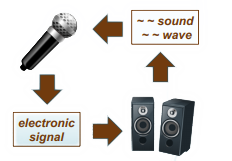
\includegraphics[width = .5\textwidth]{images/lezione9/micro_casse.png}
\end{center}

\newpage
\section{Funzionamento dei sensori}
Il compito di un sensore è quello di osservare e catturare un fenomeno fisico (onde del parlato, inquinamento in una città, ecc..) per poi tradurlo in un segnale elettrinico. Il sensore è una componente che risiede a bordo di un dispositivo il quale lo integra assieme ad altre componenti.

\section{Principali tipi di sensori}
Sensori fisici:
\begin{itemize}
    \item Sensori di movimento o inerziali: misurano le forze di accelerazione e rotazione rispetto ai diversi assi e dunque monitorano in che modo il dispositivo si muove nello spazio
    \item Sensori ambientali: Misurano parametri ambientali (fenomeni fisici) in ambiente domotico, come ad esempio la temperatura, la pressione, l'illuminazione, l'umidità, ecc
    \item sensori di posizione: misurano la posizione fisica del dispositivo. Questa categoria contiene sensori di orientamento e magnetometro
\end{itemize}
\phantom \\

Sensori virtuali:
\begin{itemize}
    \item Un dispositivo è veramente smart se è in grado di comprendere il contesto e adattarsi al fine di offrire l'obiettivo finale del sistema. In questa acquisizione di contesto partecipano i sensori posizionati sul dispositivo (fisici), ma magari si vuole sapere anche che tempo fa fuori e cosa c'è vicino al soggetto. Un esempio sono le google places api come sensori virtuali. Cosa c'è a queste coordinate? Per la risposta utilizzo una comunicazione remota tramite API. Vengono dunque ottenute informazioni tramite un web service che funge da sensore di contesto. Un'altra tipologia di sensori virtuali sono quei sensori che sono posizionati nell'ambiente attorno al dispositivo in uso e che possono essere utilizzati come se fossero installati sul dispositivo stesso. I sensori virtuali vengono considerati (dal prof) parti del sistema di sensing nonostante siano remoti.
\end{itemize}

\phantom\\

\subsection{Accelerometro e gyro}
Se i sistemi distribuiti si sono cominciati a vedere anche nella pratica per lo sviluppo delle reti, i sistemi pervasivi sono stati abilitati dallo sviluppo della sensoristica.
Il grande salto è stata la miniaturizzazione dei dispositivi e quindi una diminuzione dei costi.
\subsubsection{MEMS}
I MEMS (Micro Electro-Mechanical Systems) sono stati inventati da un'azienda nei pressi di Milano. Queste componenti harware sono state inventati per caso mentre si stavano svolgendo degli studi sulle cartucce delle stampanti. 
I MEMS sono dispositivi elettronici implementati su chip con una parte meccanica. 
Utilizzano una parte meccanica (massa e molle) per misurare l'accelerazione. Lo spostamento delle molle è misurato da una parte elettrica che misura una variazione del campo magnetico che viene generato attraverso dei condensatori. Le invenzioni di queste micro componenti ha rivoluzionato l'ambito della sensoristica e ha permesso l'implementazione a basso costo per vari dispositivi.

\subsection{Sensori ambientali}
Sensori in grado di misurare, ad esempio, il passaggio di acqua all'interno di una tubazione o il consumo energetico, etc.

\subsection{Biosensori e biosegnali}
Questa tipologia di sensoristica ha visto una nascita grazie ai MEMS per poi evolversi con dispositivi in grado di flettersi, prendendo anche la forma di cerotti o addirittura venendo integrati (sensori e attuatori) direttamente all'interno del corpo. 

\subsection{Indossabili (wearables)}
L'espansione della sensoristica e la miniaturizzazione ha permesso un'integrazione dei dispositivi indossabili in tutti i livelli. Ad esempio ci sono già stati progetti importanti della Levis con altre aziende per la creazione di indumenti sensorizzati. Ad esempio il vestito deve capire il contesto e adattare le proprietà del proprio tessuto in base all'utilità del momento. Oppure cambiare colore e proprietà. Questo ambito è ancora agli albori ed è dunque in fase di iniziale espansione.


\subsection{Beacons BLE}
I beacons sono piccoli dispositivi che emanano un segnale bluetooth low energy (BLE) i quali possono servire per localizzare un oggetto all'interno del range della tecnologia bluetooth che utilizzano. Questi dispositivi possono venire impiegati per localizzare un utente con uno smartwatch/smartphone anche in assenza di GPS, facendo triangolazioni del segnale bluetooth. La dimensione è data dalla batteria, poiché  la parte circuitale è miniaturizzata.


\subsection{Sensing device}
Il problema di questi dispotivi di sensing è che non hanno una sorgente permanente di energia e necessitano di batterie. Questi dispositivi hanno una parte di sensing subsystem, che comprende i sensori, e una power source. Questi dispositivi hanno anche le caratteristiche di un sistema distribuito: processing subsystem e wireless comunication subsystem. Hanno inoltre una minima capacità di memorizzare dati, interfacce wired per aggiornare il firmware etc, ma le cose fondamentali sono le 4 precedenti, che caratterizzano ogni dispositivo di questo genere.
\\
\\
\begin{center}
    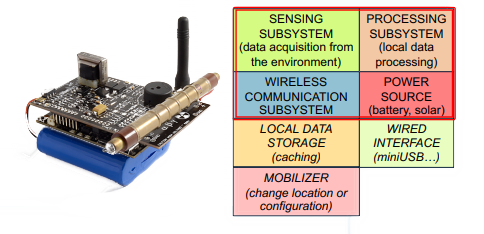
\includegraphics[width = .6\textwidth]{images/lezione9/sensing_device.png}
\end{center}

\subsection{Smartphone based sensing}
Cosa è possibile fare con l'integrazione dei dati dei sensori a bordo dei dispositivi?
Quando si sviluppano applicazioni di ogni genere bisogna avere coscienza di tutti i dati che si possono avere a disposizione. E' dunque necessario capire quali sensori sono utilizzabili dal device che l'utente avrà a disposizione perché l'applicazione sarà tanto migliore quanto sarà la sua integrazione con i sensori messi a disposizione.
\newpage
Tramite gli smartphone e i sensori posti su di essi è possibile fare inferenze su:
\begin{itemize}
    \item attività (seduto, camminando, incontra amici)
    \item mood (felice, triste)
    \item abitudini (in palestra, bar, lavoro)
    \item ambiente circostante (rumoroso, caldo, luminoso)
\end{itemize}

\subsection{SmartWatch sensing}
Questo tipo di sensing si è poi spostato anche sugli smartwatch che sono in grado di captare molte informazioni: battito puntuale, varianza nel battito, ossigenazione del sangue, tracking di attività, rumorosità dell'ambiente circostante, ecc. Molte di queste informazioni sono utilizzate poi da applicazioni lato smartphone che consigliano, in base ai valori registrati, alcune accortezze da seguire per migliorare lo stato di salute.\\
(Per capire in maniera concreta come ci si sta muovendo in questo settore, è bene informarsi sul PNRR).

\subsection{Attuatori}
Particolare tipo di trasduttore che riceve in input un segnale elettrico (dalla rete wireless) e lo trasforma in un'azione fisica. Necessitano di energia ed uno degli obbiettivi è ridurre al minimo i consumi (Esempi di azioni che compiono: Accendere la luce, aprire una porta...).

\subsection{Reti con sensori e attuatori}
Zigbee, z-wave e thread hanno un range tipico piuttosto limitato (tipicamente un ambiente casalingo), anche se possono essere estese. Hanno data rate piuttosto limitati e l'obbiettivo per cui sono state create queste tecnologie di rete è minimizzare il consumo. Funzionano a determinate frequenze (zigbee e thread usano la stessa del wifi, mentre z-wave utilizza frequenze diverse per EU e US). La topologia della rete che prevale è \textit{mesh}, in cui tutti i dispositivi vengono associati al gateway e vengono riconosciuti come partecipanti al sistema. Il dispositivo che partecipa, anche se viene spostato in una zona della casa in cui magari non riesce a raggiungere direttamente il gateway, ha comunque la possibilità di comunicare tramite procedure di heal network in cui i nodi cercano di comunicare in una modalità p2p per raggiungere il gateway utilizzando gli altri nodi come ponte. Questo rende il sistema più scalabile e più affidabile.  Sono tutte e 3 principalmente per home automation e sono concorrenti diretti. Sono state proposte varianti quali z-wave lr che dovrebbe quadruplicare il range e decuplicare il numero di dispositivi associabili nella rete. Zigbee e thread sono open source, z-wave è proprietaria. Thread (zigbee e zwave non associano un indirizzo IP al dispositivo, associano un indirizzo interno alla rete e possono essere considerati in internet attraverso l'indirizzo IP dell'abitazione, passando il comando al gateway) è stato proposto da grosse aziende ed ha l'obbiettivo di rendere ogni dispositivo IP addressable. Questa tecnologia è ottimizzata per IoT. I dispositivi in thread sono divisi in router eligible e lan device: quindi alcuni possono fare da coordinatore ed altri no, favorendo l'affidabilità.
Esiste un'iniziativa che si chiama CHIP project (connectedhome over ip)  coordinata da zigbee alliance ma a cui partecipano anche googl, amazon e apple e l'obiettivo è risucire a far interoperare dispositivi fatti da aziende diverse in una maniera quasi plug-and-play. Questo vuole essere fatto utilizzando tecnologie thread, ble e wifi integrati in una stessa rete.
\\
\\
\begin{center}
    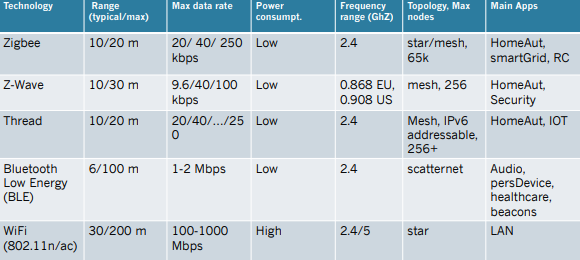
\includegraphics[width = 1\textwidth]{images/lezione9/network_sensor.png}
\end{center}
\phantom \\

\subsubsection{Base stations / Border routers}
In queste reti c'è una base station (nodo principale) che ha della potenza di calcolo e che memorizza dati in un database, acquisendoli dai sensori. Può agire come gateway tra reti (zigbee, etc) e wifi/rete internet.


\subsubsection{Discovery and pairing}
Aspetto importante degli ambienti sensorizzati è il discovery and pairing, poiché questi smart devices possono frequentemente apparire e sparire negli smart spaces e questa cosa dev'essere gestita. C'è anche una parte di netwoork bootstrapping che registra il nodo nella rete assegnandogli un indirizzo unico. L'associazione è piuttosto faticosa e particolarmente importante per quanto riguarda reti z-wave e zigbee e questa si vorrebbe semplificare con thread e nuove soluzioni. Una questione critica dell'associazione è cercare di far associare solo i dispositivi nello spazio a loro designato, anche per questioni di sicurezza. Per questo motivo si usano metodi che sfruttano sensori a bordo del dispositivo.
Scatternet: insieme di pico net connesse tra di loro. In un bluetooth lo smartphone fa da gateway bluetooth. Dall'altra parte viene visto il dispositivo bluetooth (telefono) che fa da master e le pico net fanno da slave (es. cuffie bt).


\subsection{Data acquisition}
Al fine di cambiare la temperatura in un appartamento (esempio) interrogo dei sensori. Rispetto alle query base, in questo tipo di sistemi vengono vengono utilizzate contiuos query: Ad esempio voglio sapere una certa cosa, ma il fenomeno che voglio sapere è in continua evoluzione, allora si vorrebbero effettuare delle interrogazioni che continuano a chiedere una cosa. Questo ovviamente è particolarmente oneroso in termini di chiamate. Es. Voglio sapere in maniera continua quante persone ci sono in piazza d'uomo. Modo banale: ripeto la stessa query ripetutamente in ogni momento. Questo però è troppo oneroso.
In questo ambito c'è una forte caratterizzazione spazio-temporale dei dati. 
Il problema è come interrogare di continuo senza sprecare risorse.
Metodi base
\begin{itemize}
    \item batch processing: bufferizzare i dati acquisiti dal sensore sul dispositivo ed inviare i dati alla base station o ad un server remoto. Nella base station arriverrano i dati acquisiti dai sensori e verrà effettuato un processing. Questo permette una risposta precisa, mandando i dati così come sono stati acquisiti dal dispositivo. Non viene fatto processing sul sensore. C'è però un alto costo di comunicazione. La base station riceve i dati con ritardi dovuto alla latenza etc.
    \item sampling: Non vengono inviati tutti i dati acquisiti, ma vengono inviati dati campionati. Il campionamento è fatto secondo la distribuzione attesa dei risultati in modo che siano significativi per il fenomeno che si vuole catturare. Es. Nell'audio sampling è il processo di misurare l'audio continuo ad una certa frequenza. Si considera la distribuzione attesa e lo scopo finale dei dati e così si decide il campionamento. Non offre risposta precisa, ma fornisce garanzie sull'errore che viene introdotto. Se si riesce a fare un campionamento meno frequente si risparmia nella batteria.
    \item Sliding windows: Si prende un gruppo di letture consecutive di dati e la si considera come una finestra temporale (es. finestra di 3 secondi, guardo tutti i dati, e calcolo qualcosa). Questo è il primo metodo in cui effettivamente c'è del calcolo sul dispositivo che ospita il sensore. Es: Calcolo la media delle letture e comunico alla base station il valore dell'operatore di aggregazione applicato sulla finestra. La base station riceve uno stream continuo (periodicamente) di valori approssimati con un delay poiché deve aspettare la fine della finestra, calcolare il valore aggregato e inviarlo. 
   
\end{itemize}

\subsubsection{Overlapping - Sliding windows}
Questi operatori aggregati sono chiamati features. Le window in realtà sono spesso sovrapposte (non comincia una finestra nel momento in cui finisce quella prima, bensì comincia prima che la precedente finisca). Il vantaggio della sovrapposizione consente di catturare qualcosa che sta al confine tra due finestre. Ho una maggiore qualità del dato trasmesso. Nella stragrande maggioranza dei dati inviati da sensori si utilizzano sliding windows.
\\
\\
\begin{center}
    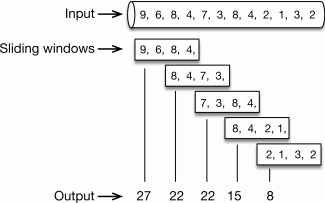
\includegraphics[width = .7\textwidth]{images/lezione9/sliding_windows.png}
\end{center}
\phantom \\






\begin{comment}
\section{Introduzione ai sensori}
Trasduttore
Sia i sensori che gli attuatori sono dei trasduttori, ossia dispositivi che trasformano una forma di energia in un'altra forma di energia.
Un esempio banale è il microfono che riceve in input delle onde sonore e manda a delle casse un segnale elettronico.
I sensori sono trasduttori di input
Gli attuatori sono trasduttori di output.

\subsection{Come funzionano i sensori}
Il compito di un sensore è quello di osservare e catturare un fenomeno fisico (onde del parlato, inquinamento in una città). Il sensore si accorge di un cambiamento fisico e lo traduce in un segnale elettronico.
Nella foto accelerometro telefono. I tre colori rappresentano i tre assi. Possiamo vedere come ci sia stato un movimento più accentuato rispetto all'asse rappresentato dalla linea blu.

\subsection{Caratterizzazione dei sensori}
\begin{itemize}
    \item Sensori fisici: 
    \begin{itemize}
        \item Sensori di movimento (inerziali): misurano le forze di accelerazione e rotazione rispetto a 3 assi.
        \item Sensori ambientali: misurano i parametri ambientali come ad esempio la temperatura, la pressione, l'illuminazione, l'umidità.
        \item Sensori di posizione: misurano la posizione fisica del dispositivo. Questa categoria contiene sensori di orientamento e magnetometro.
    \end{itemize}
    \item Sensori virtuali:
    \begin{itemize}
        \item Servizi e app che forniscono i dati sul contesto di un client remoto. Ad esempio possiamo considerare un servizio di meteo basato su termometri, anemometri, idrometri remoti e Google Places API.
    \end{itemize}
\end{itemize}

MEMS: Micro Electro-Mechanical Systems
Hanno parti elettroniche (sono installati su componenti hardware) ma anche parti meccaniche (masse e molle). 

\subsection{Biosensori e Biosegnali}
È possibile integrare questi sensori e attuatori nel corpo umano 
.....

\subsection{Wearables}
Anche indumenti e aziende di vestiti (Levis) hanno manifestato i loro interesse in queste tecnologie.

\subsection{BLE beacons}
Sono dei dispositivi (di diversa grandezza) che emanano del segnale bluetooth low energy e servono per localizzare un oggetto, sia per localizzare l'oggetto su cui è posto o tramite "triangolazioni" posso capire dove è posto un utente con il suo smartphone.

\subsection{Sensori != Dispositivi con sensori}
FOTO SLIDES

\subsection{Smarphone based sensing}
Tramite gli smartphone e i sensori posti su di essi è possibile fare inferenze su:
\begin{itemize}
    \item attività (seduto, camminando, incontra amici)
    \item mood (felice, triste)
    \item abitudini (in palestra, bar, lavoro)
    \item ambiente circostante (rumoroso, caldo, luminoso)
\end{itemize}
Questo tipo di sensing si è poi spostato anche sugli smartwatch che sono in grado di captare molte informazioni: battito puntuale, varianza nel battito, ossigenazione del sangue, tracking di attività, rumorosità dell'ambiente circostante. Molte di queste informazioni sono utilizzate poi da applicazioni lato smartphone che consigliano, in base ai valori registrati, alcune accortezze da seguire per migliorare lo stato di salute.

\section{Attuatori}
Particolare tipo di trasduttore che riceve in input segnale elettrico (dalla rete wireless) e lo trasforma in un'azione fisica.\\
Solitamente sono alimentati a batteria poichè devono svolgere un'attività fisica.

\subection{Reti con sensori e attuatori}
TABELLA

\subsection{Base station/border router/controller}
Colleziona i dati dai rilevamenti dei sensori e dagli attuatori. Può agire come gateway tra reti. Può utilizzare embedded DB. Possono trasmettere dati a unità di elaborazione.

\section{Gestire e interrogare dati dei sensori}
\subsection{Scoperta e pairing}
I dispositivi smart possono frequentemente apparire e scomparire in smart space.\\
Network bootstrapping: registrare il dispositivo alla rete e assegnare un indirizzp univoco (come per DHCP)
Associazione: associare il dispositivo ... ?

\subsection{Acquisizione dati}
\subsubsection{Metodi base}
Ci sono diversi problemi rispetto a interrogare un database tradizionale: passiamo da una one-time query a una continuous query.
\begin{itemize}
    \item Batch processing:
    \begin{itemize}
        \item Buffering suil sensore e elaborazione offline nella base station (o sul remote server)
        \item precise answer: nessuna elaborazione sul sensore, ma alto costo di comunicazione
        \item la base station riceve tutti i dati con un delay
    \end{itemize}
    \item Sampling:
    \begin{itemize}
        \item Non si mandano tutti i segnali registrati, ma solo quelli significativi
        \item ...
    \end{itemize}
    \item Sliding windows:
    \begin{itemize}
        \item Risposta approssimata basata su un gruppo di letture consecutive
        \item elaborazione run-time sul dispositivo
        \item la base station riceve uno stream cointinuato di approssimazioni di letture dal sensore
        \item Spesso le window sono overlapping. Nell'esempio ci sono delle sliding windows di dimensione 4 con overlapping del 50\%. 
        Si usa questa tecnica perchè così si evita di perdere ciò che c'è al confine tra una finestra e un'altra. Quindi in termini di comunicazione rimane uguale, migliora però la qualità del dato.
    \end{itemize}
\end{itemize}

Chicco
\subection{Metodi avanzati}
Obiettivi:
\begin{itemize}
    \item ridurre il consumo dei energia
    \item migliorare la qualità dei dati
\end{itemize}
La trasmissione consuma molta più energia che l'elaborazione. Trasmettere un bit ha lo stesso consumo di 1000 operazioni della CPU.

\begin{itemize}
    \item In-network query processing:
    \begin{itemize}
        \item Si contrappone all'elaborazione centralizzata.
        \item Si basa sulla costruzione di una overlay network
        \item aggregazione dei dati nei nodi intermedi per ridurre la trasmissione (per calcolare media, min/max, istogrammi..)
    \end{itemize}
    \item Duty cycling:
    \begin{itemize}
        \item la trasmissione è messa in un ciclo di sleep per la maggior parte del tempo
        \item ..
    \end{itemize}
    \item Mobility based:
    \begin{itemize}
        \item la base-station potrebbe essere mobile
        \item i nodi possono essere portati da persone, macchine, animali
        \item 
    \end{itemize}
    \item Model based approaches:
    \begin{itemize}
        \item 
    \end{itemize}
\end{itemize}

-------------------------------------------------------
Fabbio

\textbf{Transducer}
Sia i sensori che gli attuatori sono dei transducer. Ovvero dispositivi che trasformano una forma di energia in un'altra forma di energia. Esempio banale microfono e casse. Onde sonore che escono dalla bocca, vengono digitalizzate, arrivano dall'altra parte e un altro transducer fa il lavoro opposto. Nell'esempio della slide il microfono fa il sensore e le casse fanno da attuatori (Output transducer) 

\textbf{Come funzionano}
Il sensore è a bordo di un dispositivo che ha anche altre componenti. Il compito è quello di osservare e quindi catturare un fenomeno fisico. (Onde del parlato è un fenomeno fisico)
I sensori convertono energie in un segnale elettronico. (Nella slide output di un accelerometro) 

\textbf{Principali tipi di sensori}
Sensori fisici:
\begin{itemize}
    \item sensori di movimento o inerziali: leggi slide. Fanno un monitoraggio su come l'oggetto sul quale è monetato il sensore si muove nello spazio. (Implementati su dispositivi mobili come smartphone etc...)
    \item sensori ambientali: Nell'ambiente di domonica possono misurare dei parametri. Umidità, temperatura, luminosità... Misure di fenomeni fisici
    \item sensori di posizione: Gps. Magnetometro
\end{itemize}

\textbf{Accelerometro e gyro}
Se i sdp si sono cominciati a vedere anche nella pratica per lo sviluppo delle reti, i sistemi pervasivi sono stati abilitati dallo sviluppo della sensoristica.
Il grande salto è stata la miniaturizzazione dei dispositivi e quindi una diminuzione del costo.
I MEMS gli ha inventati un'azienda leader mondiale che stanzia vicino a milano. E' una multi nazionale che fornisce tutti i sensori all'interno dell'iphone ad esempio.
SOno stati inventati per caso studianto le cartucce delle stampanti. 
I mems sono dispositivi elettronici implementati su chip con una parte meccanica. 
Utilizza la parte meccanica (massa e molle) per misurare l'accelerazione. LO spostamento delle molle è misurato da una parte elettrica attraverso dei condensatori che misura una variazione del campo magnetico che viene generato. LE invenzioni di queste micro macchine ha rivoluzionato l'ambito della sensoristica e ha permesso l'implementazione a basso costo per vari dispositivi.

\textbf{sensori ambientali}
Possono misurare anche il passaggio di acqua, elettricità etc. 

\textbf{sensori home}
Quando si parla di home si parla di edifici e non solo di case. 

\textbf{buisensori e biosegnali}
Prima fase con i Mems che ora prosegue con dispositivi che possono essere resi flessibili anche in forma di cerotti e in altri casi è possibile integrarli nel corpo. Sensori ed attuatori che è possibile inserire nel corpo umano

\textbf{indossabili}
Un'integrazione nel wearable in tutti i livelli. QUindi anche nei vestiti. Questo ambieto è in super espansione e anche la filiera della moda è super interessata. Ci sono già stati progetti importanti della levis in tale ambito con altre aziende per la creazione di indumenti sensorizzati. Il vestito deve capire cosa succede e adatta le proprietà del tessuto a quello che serve. Oppure cambio colore e proprietà. Ambito in espansione e tutto da scoprire.

\textbf{Beacons}
Piccoli dispositivi (più piccoli stickers che sono flessibili e si possono incollare su vari oggetti) che emanano del segnale ble e possono servire per localizzare un oggetto (con il range del bluetooth). La dimensione dei beacons è data dalla batteria dato che la parte circuitale è miniaturizzata.

\textbf{sensing device}
Differenza tra sensori e dispositivo con sensori:
Il problema principale rimane la batteria perchè non hanno una sorgente permanente di energia. I dispositivi hanno una parte di sensoristica ma il dispositivo ha anche altre componenti come la batteria. 
Le cose fondamentali sono quelle della slide che caratterizzano i dispositivi di quel genere

\textbf{TIpi principali di sensori}
Virtual sensor.
Acquisizione di contesto: (un dispositivo è veramente smart se è in grado di comprendere il contesto e adattarsi al fine di offrire l'obiettivo finale del sistema) In questa acquisizione di contesto partecipano i sensori ma magari si vuole sapere anche che tempo fa fuori e cosa c'è vicino al soggetto. Un esempio sono le google places api come sensori virtuali. COsa c'è a queste coordinate? per la risposta utilizzo delle api ad esempio. Ottenere dunque informazioni tramite un web service che è come avere un sensore di contesto. Più vicini ancora sono sensori ma che non sono attaccati al nostro dispositivo, quindi il nostro dispositivo comunica con altri sensori nell'ambiente che il mio dispositivo utilizza come se fossero sensori installati sul dispositivo stesso.

\textbf{Smartphone-based sensing}
COsa si può fare con l'integrazione dei dati dei sensori a bordo dei dispositivi?
Quando si sviluppano applicazioni di ogni genere bisogna avere coscienza di tutti i dati che si possono avere a disposizione. DUnque capire quali sensori sono disponibili sul device che l'utente avrà a disposizione perchè l'applicazione sarà tanto migliroe quanto sarà la sua integrazione con i sensori messi a disposizione. 
Nella slide: Applicazione da "gande fratello" che fa vedere tutti i sensori che sta utilizzando un individuo. Cosa si può capire? L'attività che sta svolgendo, il mood che viene misurato da una proprietà elettrica che rileva uno stato di agitazione dell'utente che sta indossando il dispositivo. Es, in che zona della città si sta meglio? Posso fare degli studi su quale quartiere sia migliore.

\textbf{Smartwach sensing}
Questi tipi di sensing personali (rilevano lo stato dell'individuo e lo monitorano per molto tempo). Da questo è nato un movimento il cui obiettivo è fare da collettore di tutti i dati e darti un modo per farti stare meglio. Collezionano tanti dati e ti forniscono una soluzione su come miglirare vari aspetti della vita. Considerando sia esclusivamente personale questo aiuterebbe molto a migliorare la salute e anche in ambito di malattia per curarla in maniera più veloce e curata.
____Roba staccata dalla slide_____
Da vedere per capire in maniera concreta come ci si sta uovendo in questo ambito
PNRR: appena inviato all'unione europea. In questo piano c'è un sotto obiettivo che è la parte di telemedicina e assistenza sanitaria internazionale. Obiettivo a livello mondiale è quello di creare l'ospedale diffuso....
_________

\textbf{Attuatori}
Fanno parte della famiglia dei Transducer. Prendono il segnale elettrico, lo elaborano e lo trasformano in qualcosa di fisico nell'ambiente. (GUardare la slide che è meglio). 

\textbf{Networking con sensori e attuatori}
Come comunicano i dispositivi?
Le prime 3 hanno applicazioni tipiche in un ambiente casalingo. Hanno dei data rate limitati ma non devono comunicare chissà che cosa.
Tutti questi protocolli sono stati creati principalmente per limitatre il consumo.
Tipologia di rete che prevale: MESH
Z-Wave tecnologia proprietaria. ANche se vogliono renderlo open source per renderlo competitivo
Mesh: Nelle reti mesh anche se non tutti sono collegati tra di loro, i nodi cercano di comunicare in modo peer to peer e dunque raggiungere i nodi anche passando per altri nodi. C'è ancora una gerarchia del tipo che il gatway rimane il gateway, tuttavia i nodi si aiutano a passare i messaggi che arriveranno al gateway. Se per una qualsiasi condizione il canale diretto tra dispositivo e gateway non funziona bene, è comunque possibile passare per un altro dispositivo per raggiungere il gateway.
Nessuna delle prime due tecnologie assegnano un indirizzo ip ad ogni dispositivo.
tecnologia Thread: E' stato proposto da nestlab, samsung e altri. Ha l'obiettivo di rendere ogni dispositivo ip addressable. L'idea è che tutti i dispositivi, seppur miniaturizzati, siano tutti dotati di indirizzi ip. E' ovviamente ottimizzato per l'uso dell'Iot. I dispositivi in thread sono:
router eligible o trend device. Ci possono essere dei dispositivi che fanno da coordinatori e altri no. Più dispositivi router eligible significa maggior affidabilità.
C'è un'iniziativa che si chiama CHIP project (connectedhome over ip o qualcosa di simile)  coordinata da zigbee alliance ma partecipano google amazon e apple e l'obiettivo è risucire far interoperare dispositivi fatti da aziende diverse in una maniera quasi plug-and-play. QUesto utilizzando thread, ble e wifi integrati in una stessa rete.

\textbf{base stations/border routers}
In queste reti c'è una base stations chiamata anche border router.. .C'è un nodo principale con potenza di calcolo e con un database interno che fa da gateway tra il protocollo (tipo zigbee) e la rete wifi. 

\textbf{Discovery and pairing}
Rispetto ad un sistema distribuito in cui i nodi sono computer veri e propri, nonostante possano disassociarsi dal sistema ed entrare nel sistema, in questo cso questi smart devices possono apparire e scomparire dai sistemi.
C'e una parte di network boostrapping in cui il dispositivo viene registrato nella rete in cui viene assegnato un indirizzo unico al nodo.
Dopo la parte di associazione il nodo avrà un indirizzo unico.
L'associazione è quella procedura piuttosto faticosa (per quanto riguarda z-wave e zigbee) però è particolarmente importante. Innanzitutto la fase di associazione l'hanno sperimentata tutti con il bluetooth. 
Scatternet: insieme di pico net connesse tra di loro. In un bluetooth lo smartphone fa da gateway bluetooth. Dall'altra parte viene visto il dispositivo bluetooth (telefono) che fa da master e le pico net fanno da slave.

\textbf{Data acquisition}
Al fine di cambiare la temperatura in un appartamento (esempio) interrogo dei sensori. Rispetto alle query base, in questo tipo di sistemi venogno fatte da continuos query: Voglio sapere una certa cosa, ma il fenomeno che voglio sapere è in continua evoluzione, allora io potrei volere delle interrogazioni che continuano a chiedere una cosa. QUesto ovviamente è particolarmente costoso. Es. Voglio sapere in maniera contianua quante persone ci sono in piazza d'uomo. Modo banale: ripeto query in ogni moemnto. Questo però non è la roba migliore da fare.
In questo ambito c'è una forte caratterizzazione spazio-temporale dei dati. 
Il problema è come interrogare di continuo senza sprecare risorse.
Metodi base
\begin{itemize}
    \item batch processing: bufferizzare dati rilevati dal sensore e invio i dati ad una base station (gateway/dispositivo al quale fanno riferimento gli slave). Nella base station arriverranno dati acquisiti dai sensori e faccio un processing. Tutti i dati vengono mandati così come sono stati acquisiti dal dispositivo. Non viene fatto processing sul sensore. Alto costo di comunicazione
    \item sampling: Non mando tutti i dati acquisiti ma campionarli. Il campionamento è fatto secondo la distribuzione attesa dei risultati. Es. Nell'audio sampling è il processo di misurare l'audio continuo ad una certa frequenza. Si decide di inviare un campionamento dei dati acquisiti. Non è più una risposta perfetta come nel batch. 
    \item Sliding windows: (chiesto nel progetto) Si prende un gruppo di letture consecutive di dati, la si considera come una finestra temporale, (es. finestra di 3 secondi, guardo tutti i dati, e calcolo qualcosa). QUesto è il primo metodo conu ncalcolo sul dispositivo. Es: Calcolo la media delle letture e comunico alla base station la media che ho appplicato sulla finestra. I valori sono un'approssimazione di tutti i valori nella finestra.
    [Esempio nella slide sliding windows di un accelerometro]
\end{itemize}

\textbf{Sliding windows}
La finestra scelta nella slide è di un secondo. In un secondo il dispositivo prende le misure e calcola le features (operatori aggregati). 

\textbf{overlapping}
Si vedono finestra consecutive ma in realtà le window sono spesso overlapping. Nelle sliding window le finestre sono sovrapposte. Nella slide l'overlap è del 50 percento. Il vantaggio nell'usare l'overlapping? Riesco a non perdere dei dati tipo fenomeno che sta al confine tra due finestre.  Ho una maggiore qualità del dato trasmesso. Nella stragrande maggioranza dei dati inviati da sensori si utilizzano sliding windows

\textbf{Advanced methods - metodi avanzati}
Problema dei sistemi mobile/pervasivi è che alcuni nodi sono alimentati a batteria/pannelli solari. Bisogna dunque preoccuparsi del risparmio di energia.
Questi metodi cercano di capire se la computazione fatta dai nodi sia la trasmissione si può ottimizzare rispetto al consumo di energia.
Il focus generale al momento è sui veicoli, ma la ricerca fatta in quell'ambito va in parallelo con lo sviluppo della tecnologia dei nodi di sensing. 
Un altro obiettivo è quella di migliorare la qualità dei dati. Bisogna avere dati attendibili abbastanza significativi rispetto al fenomeno che sto osservando. La gran parte del lavoro degli algoritmi di machine learning prevede la puluzia dei dati. 
Cosa consuma di più la batteria? la trasmissione. Bisogna avere una rete che facilita il risparmi odi energia e bisogna trasmettere il meno possibile.
Il costo del sensing dipende dal sensore che si va ad utilizzare. Va valutato quindi in base ai sensori. 

Metodi avanzati 
\begin{itemize}
    \item in network-query processing: Si potrebbe organizzare la rete dei nodi (non a livello fisico, ma costruendo una rete over-lay) facendo data aggregation.  Faccio la query e la risolvo principalmente utilizzando il calcolo computazionale dei nodi 
    \item duty cycling: dico quanto deve rimanere in sliping mode il nodo prima di inviare il messaggio. Posso anche utilizzare altri paramentri per dire "invia il messaggio se succede questo".
    \item mobility-based: le base station potrebbero essere mobili e ci sono dei metodi che permettono di utilizzare la distanza andando cosi' a minimizzare il costo di comunicazione
    \item model based approches:
\end{itemize}

\textbf{Model-based approches}
L'idea è che i dati che provengono da dispositivi con sensori hanno una forte correlazione spazio temporale. (es. se ho un sensore di temperatura fisso in un certo luogo in una certa città, osservo che durante l'hanno ho dei valori che si ripetono nel tempo in ogni stagione). Allora posso modellare questa correlazione spazio temporale. Se voglio ridurre il consumo di energia devo diminuire la quantità di dati trasmessi. Come faccio?
Uso un modello (funzione) che conoscono sia la base station sia il nodo che rileva i dati. Se i dati rilevati dal nodo si allontanano dal modello (oltre una certa tolleranza), allora il nodo comunica alla base station i nuovi dati rilevati. Problema, in questo modo non sappiamo se tutto funziona correttamente dato che potrebbe essere che il nodo è crashato e quindi non invia i dati per quel motivo. Quindi si utilizzano dei messaggi di alive a basso consumo energetico per segnalare ogni tot che il nodo X è ancora operativo.
Il modello non rimane fisso nel tempo ma si può anche aggiornare, in tal caso si aggiorna e si comunica ai vari nodi il nuovo modello.
I sensori e i dispositivi che registrano sono poco affidabili in generale, quindi servono dei meccanismi che servono per cancellare il rumore dai dati. Ad esempio quando la base station riceve il dato inviato dal nodo deve capire se il dato ricevuto va considerato "buono" o meno.


\textbf{sensor data cleaning}
I dati che arrivano dal sensore spesso sono sbagliati per svariati motivi (leggi slide). Il model based data cleaning è fondamentale e i valori più attendibili sono ottenuti da modelli statistici.
(Immagine)
Il processo di data cleaning viene solitamente fatto nella base station, non sul dispositivo. (E' comunque possibile fare preprocessing sul dispositivo (nodo) qualora avesse la capacità di calcolo). - Offline e online nell'immagine dice che ci sono due diversi approcci di data cleaning. -
Stream processing engine: A cui arrivano i dati dalla rete. Nell'online l'anomaly detector analizza in tempo reale i dati. 
Alcuni dei modelli di data cleaning: principalmente regressione polinomiale

\textbf{Data acquisition}
Due modi principali.
pull-based:
L'utente fa un'interrogazione, manda una query alla base station e la base station passa l'interrogazione alla rete propria. Se è una continuos query dico di calcolare i lvalore richiesto e mandarmi periodicamente il messaggio.
push-based:
La base station manda a tutti i dispositivi il modello di calcolo (anche differenziato se sono su zone diverse). Quando un valore devia, la rete avvisa la base station. Altrimenti la base station risponde alla query secondo il modello stabilito. (?)
Differenza con il modello per data cleaning: Nell'architettura di rete la differenza d'utilizzo è che nel cleaning non c'è necessità di inviare il modello ai sensori. Sono ortogonali (?). 

\textbf{Model-based compression}
Comprimere i dati dei sensori.  Questo metodo è "indipendente". L'obiettivo è approssimare uno stream di dati con un insieme di funzioni. 
Una famiglia di metodi per fare ciò è quella dei Piecewise linear or constant approximation model. I dati che arrivano ad un sensore sono una serie temporale fatta di timestamp (asse x) e un valore (nell'esempio di temperatura). Ognno degli elementi nella fiura è un elemento della serie temporale. Un segmento è come nella sliding window. I segmenti iniziano e finiscono con una misurazione. Perchè piecewise... ? Perchè prendo tutte le misurazioni nel segmento e le approssimo con una costante. COme lo scelgo? (segmenti di diversa lunghezza perchè i modelli di compressione si basano sul definire un errore massimo definito per la ricostruzione futura dei dati. La piecewise linear approssimation sarà una retta con una certa inclinazione che modella in modolineare e non costante. Quando cambio segmento? Se capisco che i valori nuovi vanno oltre epsilon di errore, cambio segmento sperando che i valori successivi saranno più vicini al nuovo segmento.
La correlazione spazio temporale dei dati fa si che questo metodo sia ragionevole in quanto si tende a seguire un andamento. (es. abbassamento temperatura costante)
Vengono utilizzate tecniche in cui i dati che ho cambiano comportamento in maniera repentina. dunque questo può esser esteso in un multimodel in cui si cambia modello di riferimento. 

\textbf{Cloud platforms for iot and data stream processing}
Esistono tool che aiutano a fare il processing da noi intuito e che è necessario fare per l'analisi di stream che arriva dei sensori.

\textbf{Google IOT core architecture}
Fa vedere uno degli aspetti che si stanno ricercando (nell'immagine). (?)




--------------------------------------------------

Omar Wilde - lo scrittore del bestseller "Doriano Grigio"

Sia i sensori che gli attuatori sono dei transducer: un dispositivo che trasforma una forma di energia in un'altra forma di energia. Esempio banale: microfono, che funziona da sensore, e casse, che funzionano da attuatore.
Il sensore è a bordo di dispositivi con altri componenti, il suo obbiettivo è osservare e catturare un fenomeno fisico, come possono essere le onde sonore del parlato, memorizzandolo sotto forma di dati.

I sensori possono essere:
- fisici
* sensori di movimento, chiamati anche inerziali: monitoraggio di come l'oggetto sul quale è montato il dispositivo si muove nello spazio
* sensori ambientali: misurano dei parametri (fenomeni fisici) in ambiente di domotica, quali umidità, temperatura, pressione, illuminazione, ecc
* sensori di posizione: sì
- virtuali: informazioni aggiuntive sul contesto rispetto a quanto rilevato dai sensori fisici (?), ad esempio Google Places API può ritornare cosa c'è attorno rispetto ad una certa posizione. Li considero parti del sistema di sensing, ma sono remoti.

I sistemi pervasivi sono stati abilitati dallo sviluppo della sensoristica ed il grande salto è stata la miniaturizzazione di questi dispositivi (e riduzione del costo). I MEMS sono stati inventati da un'azienda multinazionale nei pressi di Milano. Sono stati inventati per caso, studiando qualcos'altro. 
Questa fase di miniaturizzazione sta proseguendo con disposistivi che possono essere flessibili e integrati nel corpo umano.

I beacons sono piccoli dispositivi che emanano del segnale bluetooth low energy e possono servire per localizzare un oggetto, compatibilmente con il range di questa tecnologia di rete, e possono localizzare un utente con uno smartwatch/smartphone anche in assenza di GPS, facendo triangolazioni del segnale bluetooth. La dimensione è data dalla batteria, poiché la parte di circuito è molto piccola.

Il problema di questi dispotivi è che non hanno una sorgente permanente di energia e necessitano di batterie. Questi dispositivi hanno una parte di sensing subsystem, che comprende i sensori, e una power source. Ha anche le caratteristiche di un sistema distribuito: processing subsystem e wireless comunication subsystem. Ha inoltre una minima capacità di memorizzare dati, interfacce wired per aggiornare il firmware etc, ma le cose fondamentali sono le 4 precedenti, che caratterizzano ogni dispositivo di questo genere.

Gli attuatori sono anch'essi un transducer, poiché prendono un segnale elettrico e lo trasformano in un'azione di modifica dell'ambiente. Necessitano di energia ed uno degli obbiettivi è ridurre al minimo i consumi.

Zigbee, z-wave e thread hanno un range tipico piuttosto limitato (tipicamente un ambiente casalingo), anche se possono essere estese. Hanno data rate piuttosto limitati e l'obbiettivo per cui sono state create queste tecnologie di rete è minimizzare il consumo. Funzionano a determinate frequenze (zigbee e thread usano la stessa del wifi, mentre z-wave utilizza frequenze diverse per EU e US). La topologia della rete che prevale è mesh, in cui tutti i dispositivi vengono associati al gateway e vengono riconosciuti come partecipanti al sistema, dopodiché il dispositivo viene spostato in una zona della casa che magari non riesce a raggiungere direttamente il gateway, quindi avvengono procedure di heal network (?) in cui i nodi cercano di comunicare in una modalità p2p per raggiungere un nodo passando attraverso un altro nodo. Questo lo rende più scalabile e più affidabile. Sono tutte e 3 principalmente per home automation e sono concorrenti diretti. Sono state proposte varianti quali z-wave lr che dovrebbe quadruplicare il range e decuplicare il numero di dispositivi associabili nella rete. Zigbee e thread sono open source, z-wave è proprietaria (?). Thread (zigbee e zwave non associano un indirizzo IP al dispositivo, associano un indirizzo interno alla rete e possono essere considerati in internet attraverso l'indirizzo IP dell'abitazione, passando il comando al gateway (?)) è stato proposto da grosse aziende ed ha l'obbiettivo di superare il limite e rendere ogni dispositivo IP addressable ed è ottimizzato per IoT. I dispositivi in thread sono divisi in router eligible e lan device: quindi alcuni possono fare da coordinatore ed altri no, favorendo l'affidabilità.

CHIP project (connect home over ip o qualcosa di simile): iniziativa da zigbee alliance a cui partecipano google e amazon, tra gli altri, con l'obbiettivo di far interoperare dispositivi di operatori diversi fatti da aziende diverse (in ambito home) in maniera quasi plug n play, utilizzando thread, bluetooth low energy e wifi, e facilitando associazione/disassociazione di dispositivi.

In queste reti c'è una base station (nodo principale) che ha della potenza di calcolo e che memorizza dati in un database, acquisendoli dai sensori. Fa da gateway tra rete dei sensori (zigbee, etc) e wifi/rete internet (?)

Aspetto importante degli ambienti sensorizzati è il discovery and pairing, poiché questi smart devices possono frequentemente apparire e sparire negli smart spaces e questa cosa dev'essere gestita. C'è anche una parte di netwoork bootstrapping che registra il nodo nella rete assegnandogli un indirizzo unico. L'associazione è piuttosto faticosa per quanto riguarda reti z-wave e zigbee che si vorrebbe semplificare con thread e nuove soluzione, che però è praticolarmente importante. Una question crtiica dell'associazione è limitare device e servizi appartenenti allo spazio fisico designato, anche per questioni di sicurezza. Per questo motivo si usano metodi che sfruttano sensori a bordo del dispositivo.

Vado ad interrogare i sensori utilizzando continuous query (db utilizzano one time query), che mi consentono di sapere una certa cosa, ma siccome il fenomeno che si sta osservando è in continua evoluzione, vorrei che questa venisse continuamente chiesta. Questo è particolarmente costoso, per cui ci sono tecniche di ottimizzazione ed una forte caratterizzazione spazio temporale dei dati. Vogloiamo quindi interrogare i sensori senza sprecare risorse.

Metodi base per prendere i dati da una rete di sensori:
- batch processing: bufferizzare i dati acquisiti dal sensore sul dispositivo ed inviare i dati alla base station o ad un server remoto. Nella base station arriverrano i dati acquisiti dai sensori e viene effettuato un processing. Questo permette una risposta precisa, mandando i dati così come sono stati acquisiti dal dispositivo, non viene fatto processing sul sensore. C'è però un alto costo di comunicazione. La base station riceve i dati con ritardi dovuto alla latenza etc.
- sampling: non mandare tutti i dati acquisiti, ma campionarli, considerando la distribuzione attesa dei valori, in modo che sia rappresentati per il fenomeno che si vuole catturare. Il campionamento ad esempio viene fatto nel suono. Si considera la distribuzione attesa, lo scopo finale dei dati e si decide il campionamento. Non offre risposta precisa, ma fornisce garanzie sull'errore che viene introdotto. Se si riesce a fare un campionamento meno frequente si risparmia nella batteria.
- sliding window: ampiamente utilizzato. Abbiamo una risposta approssimata. Qui prendiamo un gruppo di readings consecutive (nel gruppo), la consideriamo una finestra temporale e calcolo qualcosa. Primo metodo in cui effettivamente c'è del calcolo sul dispositivo che ospita il sensore. Tipicamente può calcolare la media, per esempio. Comunica alla base station il valore dell'operatore di aggregazione applicato sulla finestra. La base station riceve uno stream continuo (periodicamente) di valori approssimati con un delay poiché deve aspettare la fine della finestra, calcolare il valore aggregato e inviarlo.
Questi operatori aggregati sono chiamati features. Le window in realtà sono spesso sovrapposte (non comincia una finestra nel momento in cui finisce quella prima, bensì comincia prima che la precedente finisca). Il vantaggio della sovrapposizione consente di catturare qualcosa che sta al confine tra due finestre.

Il sensore registra il valore fisico, la composizione della finestra la fa il dispositivo che ha a bordo il sensore.

Metodi avanzati:
Hanno l'obiettivo di risolvere il problema che alcuni di questi nodi sono alimentati a batteria, dunque dobbiamo occuparci del risparmio di energia. Inoltre si vuole migliorare la qualità dei dati, cioè avere dati attendibili, abbastanza significativi rispetto al fenomeno che si sta osservando.
La trasmissione è ciò che consuma di più, occorre dunque una rete che facilità il risparmio di energia ed inoltre dobbiamo trasmettere il meno possibile. Il batch è dunque particolarmente costoso ed il meno auspicabile dal punto di vista del consumo.
La trasmissione costa molto di più del calcolo, mentre il costo del sensing può variare a seconda del sensore. L'accellerometro consumerà meno di un GPS. Tipicamente, però, dobbiamo prestare attenzione alla trasmissione.

Metodo 1:
In-network query processing: per evitare la comunicazione di tutti i dati alle station, si potrebbe costruire una rete virtuale (overlay) e fare data aggregation nei nodi intermedi per ridurre la trasmissione. Dunque, mano a mano che i componenti raccolgono i dati dai sensori e se li comunicano tra di loro, fanno delle aggregazioni intermedie. Faccio parte della query usando il potere computazionale dei nodi e non tutto con la base station, risparmiando così comunicazione, che è quella che costa.

Metodo 2:
Duty cycling: hanno un parametro sul gateway per il duty cycling, il che vuol dire che la radio sul dispositivo è in sleep mode per l'intervallo specificato. Dopo questo intervallo fa la comunicazione con il gateway e se viene modificato il duty cycling, prende quel parametro e andrà in sleep mode per quel tempo. Altre modalità permettono di far fronte a particolare esigenze con delle regole particolari sull'invio nonostante sia in sleep mode (?).

Base station possono essere mobili/nodi edge, quind esistono metodi per sfruttare la vicinanza in base alla disposizione geografica (?)

Metodo 3: approcci basati sul modello
I dati che provengono da dispositivi con sensori solitamente hanno una forte correlazione spazio-temporale, cioè posso avere un andamento che si ripete nel tempo, inoltre il cambiamento in un certo intervallo di tempo è limitato in un certo range. Questo dipende dalla proprietà che si sta osservando. Posso modellare questa correlazione in un grafico. Potremmo avere una funzione che determina la correlazione temporale con il fenomeno che sto osservando. Siccome voglio consumere il consumo di energia, riduco la quantità di dati che trasmetto, voglio però mantenere una buona qualità dei dati. Il metodo (viene usato per tante cose) si basa su:
- il gateway comunica al dispositivo la funzione, dopo aver studiato i dati ricevuti. A questo punto, sia il dispositivo che la base station hanno la funzione ed il dispotivo, per minimizzare la comunicazione, potrà comunicare il dato solo quando si allontana dal modello. Ovviamente ci vuole una certa tolleranza. Se il valore che arriva dal sensore è dentro l'intervallo delta non comunica niente. Ci sarà un keep alive, un segnale a basso imapatto energetico che assicura che il dispositivo sia ancora attivo. Si può anche decidere che ci sono dei segmenti di tempo in cui si utilizza la funzione e poi c'è una taratura.
Si studia quindi statisticamente l'andamento spzio temporale dei dati, si comunica al device e si comunica quando si esce dal delta. Applicazioni di questo:

*Questa cosa è stata applicata al data cleaning: sensori e dispositivi sono poco affidabili, per questo si tende a fare ridondanza (più sensori in una certa area). Servono meccanismi per riuscire a isolare e cancellare dati noisy. Questo discorso dei modelli viene applicato anche per questo, con delta diversi. Quando la base station riceve il dato deve capire se può considerarlo buono oppure no. Il processo di data cleaning viene solitamente fatto nel gateway/base station (dove arrivano i dati e verranno poi processati). È possibile anche fare un cleaning sul dispositivo se ne ha le capacità, altrimenti viene fatto solo su gateway che può essere elaborazione online o offline. Lo stream processing engine riceve i dati dai dispositivi che gestiscono i sensori. Questi dati vengono memorizzati nell'online immediatamente, mano a mano che arrivano. Nel stream processing engine c'è un modulo che fa l'analisi dello stream dei dati che arrivano: ha il modello statistico dei dati come dovrebbero essere, confronta anche con altri sensori nella stessa stanza, quindi con modello statistico e correlazione pulisce i dati, tenendo però comunque i dati originali in una tabella distinta da quelli puliti, poiché l'anomaly detector può anche sbagliare, dunque se cambia la funzione posso riapplicarla offline e ripulire meglio i dati. Per il data cleaning si usa principalmente la regressione polinomiale.
*query processing: la base station se arriva una query in cui dovrebbe usare un dato che non ha utilizza la funzione.
*device che devono mantenere sul device stesso parecchi dati, può utilizzare il modello per comprimere

Due modi di fare data acquisition: l'utente fa una query alla base station che passa l'interrogazione alla rete vera e propria in una modalità pull, cioè se è una continuous query dice alla rete di calcolare il valore che viene richiesto e mandare periodicamente il risultato. La push utilizza il modello e la rete quando c'è un valore che devia avvisa, altrimenti la base station risponde secondo i valori stimati dalla funzione del modello.

I modelli possono essre usati quindi in 4 modi, 2 che abbia considerato:
- data cleaning
- data acquisition
Il modello può essere lo stesso, nell'architettura la differenza tra questi due modi di usarlo sta nel fatto che nel cleaning non c'è necessità di comunicare il modello ai sensori

Ci sono modelli che riescono a catturare le correlazioni tra i diversi sensori e altri che invece fanno indipendente per ciascun sensore (lineare (indipendente (?)) e marcoviano).

Recap: l'idea degli approcci basati sul modello è che i dati che arrivano dai sensori, che tipicamente vanno a monitorare un fenomeno fisico di qualche giorno, hanno una forte correlazione spazio-temporale tra di loro ed esprimo una certa regolarità. L'idea di questi approcci è catturare questa correlazione con una funzione che può approssimare nel tmepo i dati che vengono osservati. Usato per:
- Data acquisition: Dalla base station viene comunicato l'expected behavior e i dispositivi che lo ricevono lo memorizzano e comunicano alla base station soltanto quando i valori che misurano i loro sensori vanno al di fuori del comportamento aspettato con dei meccanismi per capire che non ci siano crash o malfunzionamenti
- Cleaning: 
- Query processing: se alla base station arriva un interrogazione, posso generare questi dati senza andare ad interrogare, come invece nel modello pull, la rete di sensori e farmi spedire i dati. Sulla base station calcolo direttamente il risultato della query, sapendo che non sono stati spediti perché non si discostano.

Sensori possono produrre dati ad una frequenza maggiore di quella necessaria. Potremmo voler memorizzare questi dati per far processing in differita. Si possono il problema di come comprimere i dati che arrivano dal sensore, o addirittura comprimerli direttamente sul sensore per poi inviarli compressi in un tempo successivo. Può essere sfruttata l'idea del modello. L'obiettivo è approssimare uno stream di dati con un insieme di funzioni. Una famiglia di metodi per fare questa pprossimazione di stream di dati è quella dei piecewise linear or constant approximation models. Piecewise vuol dire a pezzetti. Quello in figura è il constant. I punti neri sono i valori prodotti dal sensore. I dati che arrivano da un sensore sono una serie temporale, formata da un timestamp e un valore (di temperatura in qusto caso). Ogni punto è un elemento della serie temporale. Un segmento è un certo numero di misurazioni nella time series. I segmenti iniziano e finiscono con una misurazione. Approssimo le misurazioni in un segmento con una costante. I segmenti hanno dimensione diverse poiché si basano sul definire un errore massimo consentito nella ricostruzione dei dati rappresentato con un valore epsilon. La massima distanza tra i valori della time series e 2epsilon. Cambia il segmento quando i valori vanno oltre a epsilon dal valore costante. Se i dati non avessero una forte correlazione spazio temporale un sistema del genere non funzionerebbe.

L'obiettivo è approssimare con un insieme di funzioni. Nel caso precedente potrei avere rette diverse per diversi segmenti, ma addirittura sono state proposte delle tecniche nel caso in cui ho dati che cambiano il comportamento in un modo significativo, quindi in un certo intervallo di tempo sono modellabili con delle funzioni e in un altro periodo di tempo con funzioni diverse. In ogni riga della tabella ho un puntatore al modello. 

In un contesto professionale esistono framework come Amazon AWS IOT, Google Cloud IOT e Apache Flink per fare processing per l'analisi degli stream di dati che arrivano dai sensori. 


\end{comment}